\documentclass[11pt,A4]{article}
\usepackage[T1]{fontenc}
\usepackage[utf8]{inputenc}
\usepackage[UKenglish]{babel}
\usepackage{mathtools}
\usepackage{amsthm}
\usepackage{amssymb}
\usepackage{manfnt}
\usepackage{marginnote}
\usepackage[dvipsnames]{xcolor}
%\usepackage{mathrsfs}
\usepackage[mathscr]{euscript}
\usepackage{enumitem}
\usepackage{tikz-cd}
\usepackage{hyperref}
\usepackage[noabbrev]{cleveref}
\usepackage{todonotes}
\usepackage{bbm}
\usepackage{caption}
\usepackage{subcaption}

% Plain theorems
\theoremstyle{plain}
\newtheorem{thm}{Theorem}[section]
\newtheorem{lm}[thm]{Lemma}
\newtheorem{prop}[thm]{Proposition}
\newtheorem{cor}[thm]{Corollary}

% Definition theorems
\theoremstyle{definition}
\newtheorem{defn}[thm]{Definition}
\newtheorem{nota}[thm]{Notation}
\newtheorem{exa}[thm]{Example}
\newtheorem{pbl}[thm]{Problem}
\newtheorem{q}[thm]{Question}

% Remark theorems
\theoremstyle{remark}
\newtheorem{rem}[thm]{Remark}
\newtheorem{exe}[thm]{Exercise}

% Mathbb
\newcommand{\N}{\mathbb{N}}
\newcommand{\Z}{\mathbb{Z}}
\newcommand{\Q}{\mathbb{Q}}
\newcommand{\R}{\mathbb{R}}
\newcommand{\1}{\mathbbm{1}}
\newcommand{\C}{\mathbb{C}}
\renewcommand{\P}{\mathbb{P}}
\newcommand{\CP}{\mathbb{CP}}
\newcommand{\bbE}{\mathbb{E}}
\newcommand{\bbD}{\mathbb{D}}
\newcommand{\cbbD}{\bar{\mathbb{D}}}

% Mathscr for categories
\newcommand{\scrC}{\mathscr{C}}
\newcommand{\Top}{\mathscr{T}op}
\newcommand{\CHaus}{\mathscr{CH}aus}
\newcommand{\CG}{\mathscr{CG}}
\newcommand{\Ab}{\mathscr{A}b}
\newcommand{\Set}{\mathscr{S}et}
\newcommand{\D}{\mathscr{D}}
\newcommand{\Db}{\mathscr{D}^{\mathrm{b}}}
\newcommand{\QCoh}{\mathscr{QC}oh}
\newcommand{\Coh}{\mathscr{C}oh}

% Mathcal for sheaves
\newcommand{\calC}{\mathcal{C}}
\newcommand{\F}{\mathcal{F}}
\newcommand{\G}{\mathcal{G}}
\renewcommand{\L}{\mathcal{L}}
\newcommand{\M}{\mathcal{M}}
\renewcommand{\O}{\mathcal{O}}
\newcommand{\U}{\mathcal{U}}

% Math operators
\DeclareMathOperator{\Hom}{Hom}
\DeclareMathOperator{\Cond}{Cond}
\DeclareMathOperator{\Ob}{Ob}
\DeclareMathOperator{\im}{im}
\DeclareMathOperator{\coker}{coker}
\DeclareMathOperator{\PSh}{PSh}
\DeclareMathOperator{\Sh}{Sh}

% New commands
\newcommand{\pe}{*_{pro\acute et}}
\renewcommand{\u}[1]{\underline{#1}}
\newcommand{\ot}{\otimes}
\newcommand{\op}{\oplus}
\newcommand{\fp}[1]{\times_{#1}}
\newcommand{\id}{\mathrm{id}}
\newcommand{\ev}{\mathrm{ev}}
\newcommand{\grd}{^{\bullet}}
\newcommand{\db}{\marginnote{\dbend}}


\title{Various lecture notes}
\author{Pedro Núñez}
\date{\today}

\begin{document}

\maketitle

\tableofcontents

\section{About these notes}

The purpose of these notes is to keep the material seen in lectures a bit organized and easily accesible from one single place, but they don't intend to be complete and they will surely be full of typos and mistakes\footnote{If you find any, please let me know! You can do this from GitHub or write me an email directly at pedro.nunez[at]math.uni-freiburg.de.}.

If interesting questions occur during the lectures they will be reflected here in \textcolor{blue}{blue color}.
If I want to add anything which was not said in the lecture, I will use \textcolor{ForestGreen}{green color} instead.

Warnings will be marked with a \href{https://en.wikipedia.org/wiki/Bourbaki_dangerous_bend_symbol}{dangerous bend} symbol on the margin \db.

\section{[CM] Talk 1 (Johan Commelin): Condensed Sets - 21.10.19}

\subsection{Introduction}

One of the main motivations for condensed mathematics is that topological algebraic objects have usually poor categorical and functorial properties.
For instance, topological abelian groups do not form an abelian category:

\begin{exa}
    $\R_{disc}\to \R$ is epi and mono, but not iso.
\end{exa}

Another motivation is coherent duality:

\begin{thm}
    Let $f\colon X\to Y$ be a proper or quasi-projective morphism of Noetherian schemes of finite Krull dimension. Then there exists a right adjoint $f^{!}$ to the derived direct image functor $f_{!}=Rf_{*}\colon \Db(\QCoh(X))\to \Db(\QCoh(Y))$.
\end{thm}

At some point analytic rings will come up.
We will then look at the category of solid modules, in which the 6-functor formalism works nicer than in the classical setting (e.g. when $f_{!}$ is not defined in the classical setting, $f_{!}$ takes non-discrete values in the condensed settings, which are "not there" in the classical setting).

\begin{defn}
    Pro\'{e}tale site of a point, denoted $\pe$, is the category of profinite sets with finite jointly surjective families of continuous maps as covers.
    A \textit{condensed set} (resp. group, ring, ...) is a sheaf of sets (resp. groups, rings, ...) on $\pe$.
    We denote by $\Cond(\scrC)$ the category of condensed objects of a category $\scrC$.
\end{defn}

\begin{defn}
    A \textit{condensed set} (resp. group, ring, ...) is a contravariant functor $X$ from $\pe$ to the category of sets (resp. groups, rings, ...) such that 
    \begin{enumerate}[label=\roman*)]
	\item $X(\varnothing)=*$.
	\item For all profinite sets $S_{1}$ and $S_{2}$ the natural map
	    \[ X(S_{1}\sqcup S_{2})\to X(S_{1})\times X(S_{2}) \]
	    is an isomorphism.
	\item For any surjection of profinite sets $f\colon S'\twoheadrightarrow S$ we get an induced\footnote{Since the pullback diagram is commutative, the image of $X(f)$ is indeed induces a morphism as claimed.} isomorphism
	    \[ X(S)\to \{ x\in X(S')\mid \pi_{1}^{*}(x)=\pi_{2}^{*}(x)\in X(S'\fp{S}S')\} \]
    \end{enumerate}
\end{defn}

We will call $X(*)$ the \textit{underlying object} in $\scrC$ of a condensed object.

\begin{rem}
    We will use $T$ for topological spaces vs. $X,Y$ for condensed sets, as opposed to Scholze's mixing of those notations.
\end{rem}

\subsection{Recollections on sheaves on sites}

Let $F$ be a presheaf on a site, which is just a contravariant functor to whatever category in which our sheaves are gonna take values.
If $U=\cup_{i}U_{i}$ is an open cover, the topological sheaf axiom could be phrased as: $F(U)$ is an equalizer of the diagram
\[ \prod_{i}F(u_{i})\rightrightarrows \prod_{i,j}F(U_{i}\cap U_{j}). \]
Note that $U_{i}\cap U_{j}$ is just the fiber product of the two inclusions.

\begin{defn}[Coverage]
    See definition 2.1 in \href{https://ncatlab.org/nlab/show/coverage}{nCat}.
\end{defn}

\begin{defn}
    $F$ a presheaf on $\scrC$.
    A collection $(s_{i})\in \prod_{i}F(U_{i})$ for $\{f_{i}\colon U_{i}\to U\}$ a covering is called a \textit{matching family} if for all $h\colon V\to U$ we have $g^{*}(s_{i})=h^{*}(s_{j})$ for $g$ and $h$ in the diagram
    \begin{center}
	\begin{tikzcd}
	    V\arrow{r}{h}\arrow{d}{g} & U_{j}\arrow{d}{f_{j}} \\
	    U_{i}\arrow{r}{f_{i}} & U
	\end{tikzcd}
    \end{center}
\end{defn}

\begin{defn}
    $F$ is a sheaf with respect to $\{U_{i}\to U\}$ if for all matching families $(s_{i})$ there exists a unique $s\in F(U)$ such that $f_{i}^{*}(s)=s_{i}$.
    We say that $F$ is a \textit{sheaf} if it is a sheaf for all covering families.
\end{defn}

\begin{rem}
    A sheaf of abelian groups is just a commutative group object in the category of sheaves of sets.
\end{rem}

\begin{thm}
    If $\scrC$ is a site, then $\Ab(\scrC)$ is an abelian category.
\end{thm}

\begin{defn}
    An additive category is a category in which the hom-sets are endowed with an abelian group structure in a way that makes composition bilinear and such that finite biproducts exist.
\end{defn}

Recall Grothendieck's axioms:
AB1) Every morphism has a kernel and a cokernel.
AB2) For every $f\colon A\to B$, the natural map $\operatorname{coim}(f)\to \im{f}$ is an iso.
AB3) All colimit exist.
AB4) AB3) + arbitrary direct sums are exact.
AB5) AB3) + arbitrary filtered colimits are exact.
AB6) AB3) + $J$ an index set, $\forall j\in J$ a filtered category (think of directed set) $I_{j}$, functors $M\colon I_{j}\to \scrC$, then
\[\varinjlim_{(i_{j}\in I_{j})_{j}}\prod_{j} M_{i_{j}}\to \prod_{j\in J}\varinjlim_{i_{j}\in I_{j}} M_{i_{j}} \]

\begin{thm}
    $\scrC$ a site. Then $\Ab(\scrC)$ satisfies AB3), AB4), AB5) and AB6).
\end{thm}

In fact, our case is even nicer:

\begin{thm}
    $\Cond(\Ab)$ in addition satisfies AB6) and AB4*).
\end{thm}

\subsection{Compactly generated topological spaces}

\begin{defn}
    A topological space $T$ is called \textit{compactly generated} if any function $f\colon T\to T'$ is continuous as soon as the composite $S\to T\to T'$ is continuous for all maps $S\to T$ where $S$ is compact and Hausdorff.
    See also \href{https://ncatlab.org/nlab/show/compactly+generated+topological+space}{nCat}.
\end{defn}

The inclusion functor $\CG \hookrightarrow \Top$ has a right adjoint $(-)^{cg}$.
If $T$ is any topological space, then the topology on $T^{cg}$ is the finest topology on $T$ such that $\sqcup_{S\to T}S\to T$ is continuous, where $S$ ranges over all compact Hausdorff spaces.

Let $T$ be a topological space.
We view $T$ as a presheaf on $\pe$ by setting $T(S)=\Hom_{\Top}(S,T)$ for all profinite sets $S$.
We denote this by $\u{T}$.
Claim: $\u{T}$ is a sheaf.
\begin{enumerate}[label=\roman*)]
    \item The first condition $\u{T}(\varnothing)=*$ is true, because there is exactly one morphism from the empty set to any topological space.
    \item $\u{T}(S_{1}\sqcup S_{2})=\u{T}(S_{1})\times \u{T}(S_{2})$ by universal property of disjoint union.
    \item For any surjection $S'\twoheadrightarrow S$ we get an isomorphism
	\[ \u{T}(S)\to \{ x\in \u{T}(S')\mid \pi_{1}^{*}(x)=\pi_{2}^{*}(x)\in \u{T}(S'\fp{S}S')\}\]
\end{enumerate}

Since $\Top\to \Cond(\Set)$ preserves products, group objects are preserved, so it maps topological groups to condensed groups etc.

\begin{prop}
    \begin{enumerate}[label=\roman*)]
	\item This functor is faithful and fully faithful when restricted to the full subcategory of compactly generated spaces.
	\item It admits a left adjoint $X\mapsto X(*)_{top}$ where $X(*)_{top}$ gets the quotient topology of $\sqcup_{S\to X}S\to X(*)$ as above.
	    The counit $I(*)_{top}\to T$ agrees with $T^{cg}\to T$.
    \end{enumerate}
\end{prop}

Coming back to our original example:

\begin{exa}
    $\mathbb{R}_{disc}\to \mathbb{R}$ can be seen in the condensed world as $\u{\mathbb{R}_{disc}}\to \u{\mathbb{R}}$, i.e. from locally constant functions to continuous functions.
    This is still a mono, but now it is not an epi.
    The cokernel $Q$ can be described as $Q(S)=\{ S\to \mathbb{R}\text{ continuous }\}/\{ S\to \mathbb{R}\text{ locally constant }\}$.
    Note in particular that the underlying set of $Q$ is just $*$, reflecting the fact that the cokernel was trivial in the classical setting.
\end{exa}

\section{[LT] Lecture 1 - 22.10.19}

\subsection{Introduction and overview of the course}

An \textit{algebraic variety} is the solution set of a family of polynomial equations in $\C^{n}$.
For example, if $f(x,y,z,t)=xy-tz$, then
\[ V(f)=\{(x,y,z,t)\in \C^{4}\mid xy-tz=0\} \]
is an algebraic variety in $\C^{4}$.
Another example would be the parabola $\{ y-x^{2}=0\}\subseteq \C^{2}$.

Let us focus on $V(f)$ and set $t=1$.
Then $X=V(f)\cap \{ t=1 \}=\{(x,y,z)\in \C^{3}\mid xy=z\}$ can be seen as a family of complex curves parametrized by the variable $z$.
For $z=0$, the complex curve $X_{0}$ has an \textit{ordinary double point} at the origin:

\begin{figure}[h]
    \centering
    \includegraphics[scale=.5]{odpfiber}
    \caption{Topological picture of our ODP.}
    \label{fig:odpfibre}
\end{figure}

Singularities arise naturally while studying the topology of algebraic varieties, and ODP's are a particularly nice kind of singularities.

For $z\neq 0$ we get an equation which looks like $xy=1$.
In this case we have the following picture:

\begin{figure}[h]
    \centering
    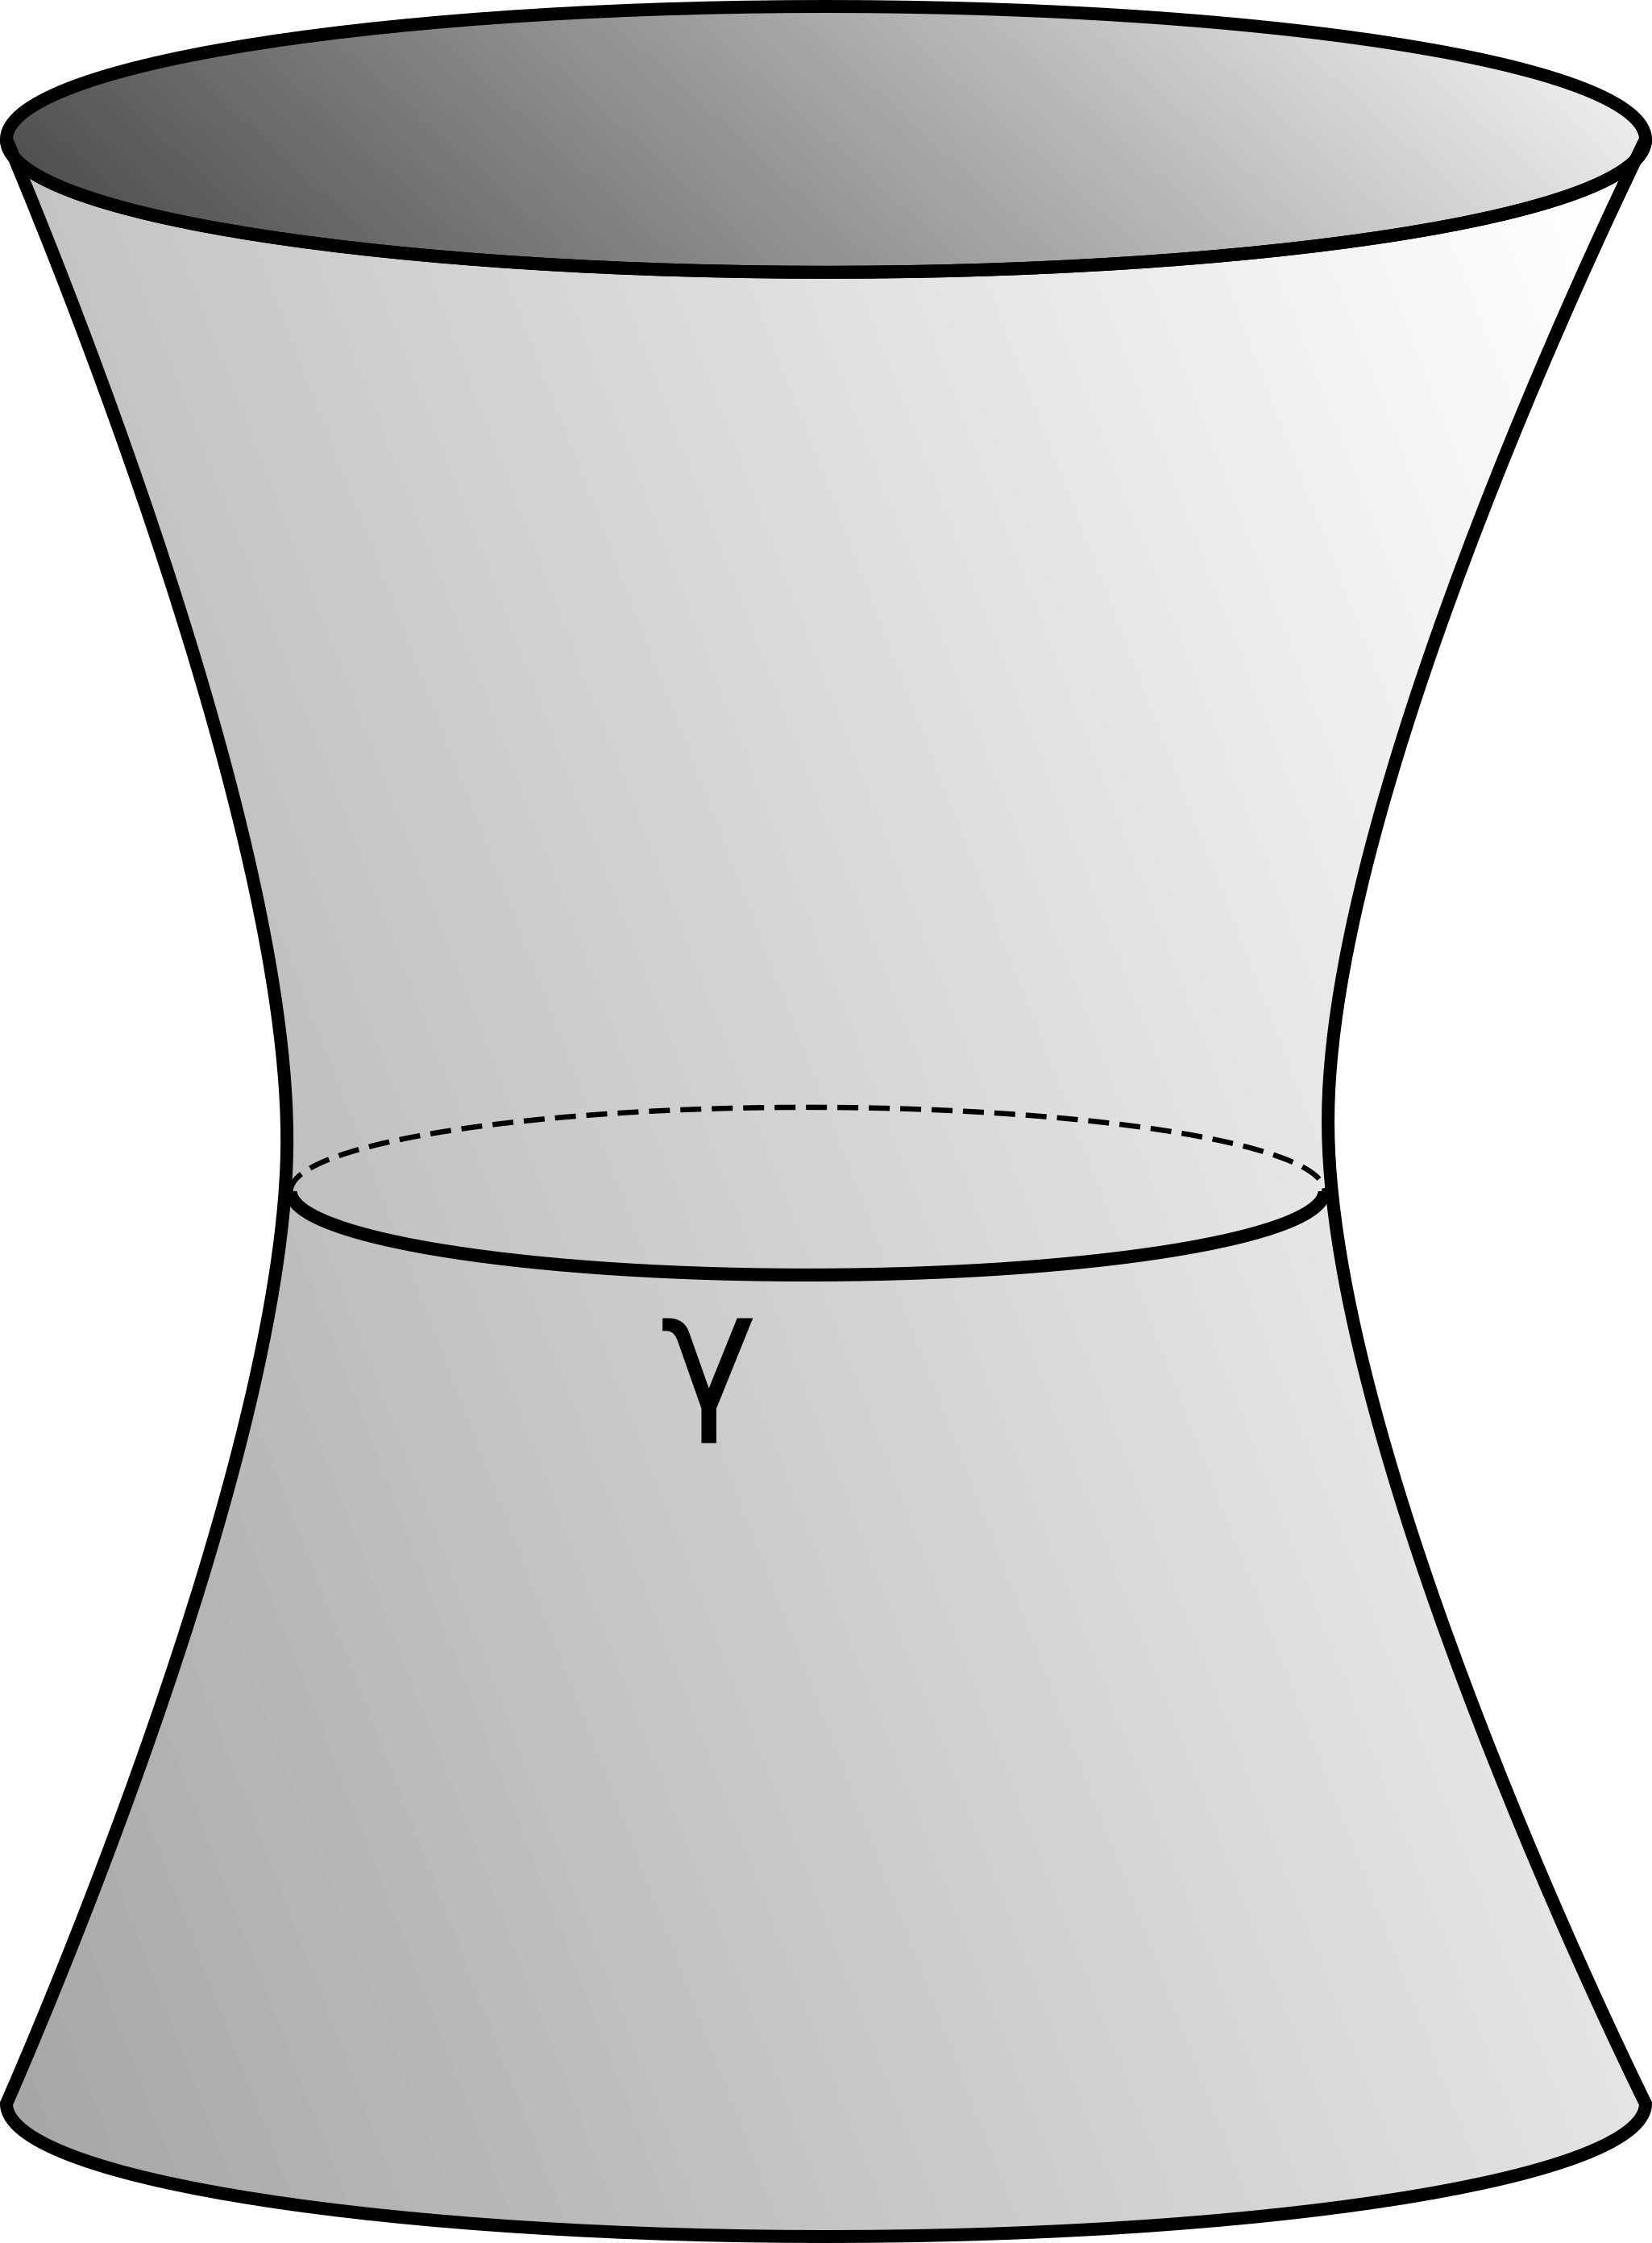
\includegraphics[scale=.8]{smoothfiber}
    \caption{Topological picture of $X_{z}$.}
    \label{fig:smoothfibre}
\end{figure}

As $z\to 0$, the central loop $\gamma$ contracts to the ordinary double point.
Note in particular that $X_{0}$ has trivial fundamental group (hence trivial $1$-homology), whereas $X_{z}$ does not.

We have a projection $\pi\colon X\to \C$, and Ehresmann's lemma tells us that for all disks $D\subseteq \C$ not containing $0$ we have $\pi^{-1}(D)\cong D\times X_{z_{0}}$ for any $z_{0}\in D$.

\begin{q}
    Given an arbitrary nonsingular algebraic variety $X\subseteq \C^{n}$, can we find a map $\pi\colon X\to \C$ such that the fibers $X_{t}$ are nonsingular for all but finitely many $t\in \C$ and such that the singular fibres have at worst ODP singularities?
\end{q}

Notice how we are missing information at infinity, e.g. $y=x^{2}$ versus $xy=1$.
The solution is to this is to replace $\C^{n}$ by $\CP^{n}$.

So let $X\subseteq\mathbb{P}^{n}$ be a nonsingular projective variety.
Then we have:

\begin{thm}
    There exists a family $(H_{t})_{t\in \CP^{1}}$ of hyperplanes in $\CP^{n}$ with $H_{[a,b]}=aH_{0}+bH_{\infty}$ such that
    \begin{enumerate}
	\item $X\subseteq \bigcup_{t\in \CP^{1}}H_{t}$.
	\item $X_{t}=X\cap H_{t}$ is nonsingular except for finitely many critical values of $t$.
	\item $X_{t}$ has ODP singularities for each critical value $t$.
    \end{enumerate}
\end{thm}

We call $(X_{t})_{t\in \CP^{1}}$ a \textit{Lefschetz pencil}.
We get a rational map $X\dashrightarrow \CP^{1}$ sending $x\mapsto t$ whenever $x\in X_{t}$.
If $x\in X_{t}\cap X_{t'}$ for $t\neq t'$, then $x\in H_{0}\cap H_{\infty}$, so this rational map is not well-defined along $X\cap H_{0}\cap H_{\infty}$.
Blowing-up this subvariety of $X$ we resolve the indeterminacy of the rational map and get a morphism $\tilde{X}\xrightarrow{\pi} \CP^{1}$ as we wanted.

As an application we obtain:

\begin{thm}[Lefschetz Hyperplane theorem]
    $X\subseteq Y\subseteq \CP^{N}$ nonsingular varieties with $X$ a hypersurface in the $n$-dimensional variety $Y$, then
    \[ H_{*}(X)\to H_{*}(Y) \]
    is an isomorphism for $*<n-1$ and a surjection for $*=n-1$.
\end{thm}

In particular, if $Y=\CP^{n}$, we have
\[ H_{*}(\CP^{n})=\begin{cases} \Z & \text{if } $*$ \text{ is even,} \\ 0 & \text{ otherwise.} \end{cases}\]
If $X\subseteq \CP^{n}$ is a nonsingular hypersurface, then its homology will be that of projective sapce on all degrees other than $n-1$.
Its $n-1$ homology will depend on the variety, e.g. the ODP (trivial $1$-homology) vs the ruled surface (with $\gamma$ non trivial on $1$-homology) from before.

\begin{exa}
    $X$ elliptic curve in $\CP^{2}$ given by $y^{2}=x(x-1)(x-\lambda)$ for $\lambda\neq 0$.
    Let $L=\CP^{1}\subseteq \CP^{2}$ and $P\in \CP^{1}\setminus (X\cup L)$.
    We get $X\xrightarrow{\pi}\CP^{1}$ by projecting from $P$ to $L$.
\end{exa}

\section{[WS] Kodaria 1 (Jin Li) - 23.10.19}

\subsection{Chow's theorem}

Let $G_{i}=G_{i}(z_{1},\ldots,z_{n})$ be homogeneous polynomials of degree $d_{i}$ for $i\in \{1,\ldots,k\}$.
Let $V=V(G_{1},\ldots,G_{k})=\{w\in \C^{n+1}\setminus \{0 \}\mid G_{i}(w)=0 \text{ for all }i\in \{1,\ldots,k\}\}\subseteq \CP^{n}$.
Assume $(\frac{\partial G_{i}}{\partial z_{j}}(w))$ is surjective at any $w\in V$.
\[ \sum_{j=0}^{n}z_{j}\frac{\partial G_{i}}{\partial z_{j}}=d_{i}G(z_{0},\ldots,z_{n}), \]
if $\tilde{w}=(\tilde{z}_{0},\ldots,\tilde{z}_{n})\in V$.
\[ \sum_{j=0}^{n}\tilde{z}_{j}\frac{\partial G_{i}}{\partial z_{j}}|_{\tilde{w}}=0\]
$V\cap U_{i}$ for any $i\in \{0,\ldots,n\}$, $U_{i}=\{[z_{0}:\ldots:z_{n}]\in \CP^{n}\mid z_{i}\neq 0\}$.

For $i=0$, consider the chart $(U_{0},\phi_{0})$ with $\phi_{0}\colon U_{0}\to \C^{n}$ given by $[z_{0},\ldots,z_{n}]\mapsto (\frac{z_{1}}{z_{0}},\ldots,\frac{z_{n}}{z_{0}})$.
The inverse has a lift given by $\tilde{\psi}\colon \C^{n}\to \C^{n+1}\setminus \{0\}$ given by $(w_{1},\ldots,w_{n})\mapsto (1,w_{1},\ldots,w_{n})$.
\begin{center}
    \begin{tikzcd}
	\C^{n}\arrow{d}{\tilde{\psi}}\arrow{dr}{G\circ \tilde{\psi_{0}}} & \\
	\CP^{n}\arrow{r}{G} & \C^{k}
    \end{tikzcd}
\end{center}
$V\cap U_{0}=G^{-1}(\{0\})$.

$G\circ \tilde{\psi_{0}}\colon (w_{1},\ldots,w_{n})\mapsto (G_{1}(1,w_{1},\ldots,w_{n}),\ldots,G_{k}(1,w_{1},\ldots,w_{n}))$.
\[ \frac{\partial (G_{i}\circ \tilde{\psi_{0}})}{\partial w_{j}} = \frac{\partial G_{i}}{\partial z_{l}}\frac{\partial(\tilde{\psi_{0}})^{l}}{\partial w_{j}}|_{(\tilde{w_{1}},\ldots,\tilde{w_{n}})} \]
Call the LHS $A_{1}$.
\begin{equation}
    \frac{\partial G_{i}}{\partial z_{l}}|_{\tilde{w}=(1,\tilde{w}_{1},\ldots,\tilde{w}_{n})}\begin{pmatrix} 1 \\ \tilde{w}_{1} \\ \vdots \\ \tilde{w}_{n} \end{pmatrix} = 0
\end{equation}
Note also that
\[\frac{\partial (\tilde{\psi_{0}})^{l}}{\partial w_{j}}=\begin{pmatrix} 0 & \ldots & 0 \\ 1 & \ldots & 0\\ \vdots & & \vdots \\ 0 & \ldots & 1 \end{pmatrix}.\]

Now
\[(\frac{\partial G_{i}}{\partial z_{l}})=(a_{il})=\begin{pmatrix} a_{10} & \ldots & a_{1n} \\ \vdots & & \vdots \\ a_{k0} & \ldots & a_{kn}\end{pmatrix}\]
\[A_{1}=\begin{pmatrix} a_{11} & \ldots & a_{1n} \\ \vdots & & \vdots \\ a_{k1} & \ldots & a_{kn} \end{pmatrix}\]
Since $A$ is surjective and 
\[A\begin{pmatrix} 1 \\ \tilde{w}_{1} \\ \vdots \\ \tilde{w}_{n}\end{pmatrix}=0,\]
hence $A_{1}$ is surjective.

\begin{thm}[Chow]
    Every analytic closed subvariety $V\subseteq \CP^{n}$ is the zero locus of finite number of homogeneous polynomials.
\end{thm}

For this we will use as a black box:

\begin{lm}[Remmert-Stein]
    $U\subseteq \C^{n}$ domain, $S$ an analytic subvariety of $U$ of $\dim=m$, $W$ an analytic subvariety of $U\setminus S$ such that $\dim_{p}W>m$ for all regular points $p\in W$.
    Then $\bar{W}$ is analytic.
\end{lm}

Now we can prove Chow's theorem.
Suppose $\pi\colon \C^{n+1}\setminus \{ 0\}\to \CP^{n}$ has rank $n$ everywhere.
Then $\pi^{-1}(V)$ has dimension at least $1$ everywhere in $\C^{n+1}\setminus \{0 \}$ ($\pi^{-1}(V)$ is a cone missing the origin, so its closure is $\pi^{-1}(V)\cup \{0\}$).
$S=\{0\}$, $W=\pi^{-1}(V)$. 
Then $V'=\bar{W}=\pi^{-1}(V)\cup \{0\}$ is an analytic variety of $\C^{n+1}$.
Consider $V'$ near $0$.
$V'_{0}=U_{\varepsilon}(0)\cap V'$.
$V'_{0}=V(g_{1},\ldots,g_{k})$ with $g_{i}$ holomorphic on $U_{\varepsilon }(0)$.
Expand $g_{i}$ into a homogeneous polynomial $g_{i}=\sum_{n=1}^{\infty} g_{i,n}$.
Then $g_{i}(tz)=\sum_{n=1}^{\infty}g_{i,n}(z)t^{n}$ for all $x\in \C^{n+1}$ and all $t\in \C$.
If $z\in V'$, then $tz\in V'$ for all $t$.
So $g_{i}(tz)\equiv 0$ implies $g_{i,n}(z)=0$ for all $i,n$.
So $V_{0}'=V(\{g_{i,n}\})$.
By Noetherianity, finitely many $g_{i,n}$ suffice.
$V_{0}=V(g^{(1)},\ldots, g^{(m)})$.
Hence $V=V(\{ g^{(1)},\ldots, g^{(m)}\})$ in $\CP^{n}$, and this finishes the proof.

\subsection{Sheaves}

For precise definitions and results in this subsection see Wikipedia, Stacks or nLab.

Definition of \textit{sheaf} (of abelian groups) on a topological space $X$, \textit{stalk} of a sheaf at a point $x\in X$, \textit{germs} of a sheaf at a point... Note the similarities in terminology with plants.

\begin{exa}
    Constant sheaves $\Z,\Q,\R,\C$.
    Sheaf of smooth functions $\calC^{\infty}$ and its units $\calC^{*}$.
    Sheaf of regular functions $\O$ and units $\O^{*}$.
    Sheaf of meromorphic functions $\M$ and $\M^{*}$.
\end{exa}

Maps between sheaves, their kernels and their cokernels.
Short exact sequences of sheaves.

\begin{exa}
    Let $M$ be a complex manifold.
    The sequence
    \[ 0\to \Z\to \O\xrightarrow{\exp} \O^{*}\to 0 \]
    is exact.
\end{exa}

Definition of \v{C}ech cohomology of a sheaf $\F\in \Sh(M)$ with respect to an open cover $\U$, which we denote by $H^{p}(\U,\F)$ on degree $p$, and \v{C}ech cohomology of the sheaf $F$ as their direct limit over refinements, denoted $\check{H}^{p}(M,\F)$.

\begin{thm}[Leray]
    If $\U$ is an acyclic cover, i.e. if there are no higher \v{C}ech cohomologies with espect to this cover, then the \v{C}ech complex associated to this cover computes \v{C}ech cohomology.
\end{thm}

Long exact sequence in \v{C}ech cohomology induced by a short exact sequence of sheaves.

\subsection{A bit of Hodge theory}

Decomposition of the tangent space at a point of a complex manifold, its tensor algebras, $\partial $ and $\bar{\partial }$ operators, Dolbeault cohomology groups, harmonic and Hodge decomposition..
See \cite{gh78} or \cite{voi07}.

\section{[LT] Lecture 2 - 24.10.19}

\begin{rem}
    Exercise sessions will be Thursday from 13h to 15h on SR318 (Starting next week).
\end{rem}

As pointed out last week, we want to look at polynomials and their solutions sets.
But polynomials are a bit too rigid.
Instead, we look at polynomials as truncated power series, or more generally as \textit{analytic functions}, which are functions which locally can be represented as power series.
We will see that these are the same as holomorphic functions.
In particular, every holomorphic function is $C^{\infty}$.
\begin{multline*}
    \text{polynomials} \Rightarrow \text{convergent power series} \Rightarrow \text{analytic} \Leftrightarrow \\
    \Leftrightarrow \text{holomorphic} \Rightarrow C^{\infty}\Rightarrow \text{continuous} \Rightarrow \text{abominations}
\end{multline*}

If we were analysts we would start at the bottom and then try to swim up.
Instead we will start from the top and float downstream.

\begin{nota}
    $\bbE=\R$ or $\C$.
    $z=(z_{1},\ldots,z_{n})\in \bbE^{n}$, $r\in \R_{\geqslant 0}$.
    Recall
    \[ |z|=\sqrt{2}{z_{1}\bar{z_{1}}+\cdots + z_{n}\bar{z_{n}}}, \]
    \[ \bbD(z,r)=\{w\in \bbE^{n}\mid |z-w|<r\}, \text{ and} \]
    \[ \cbbD(z,r)=\{ w\in \bbE^{n}\mid |z-w|\leqslant r\} \]
    called oepn and closed disks respectively.
    We call $\cbbD(z_{1},r_{1})\times \cdots \times \cbbD(z_{n},r_{n})$ an \textit{open polydisk}.
\end{nota}

\subsection{Formal power series}

\begin{defn}
    Let $a=(a_{1},\ldots,a_{n})\in \C^{n}$.
    A \textit{formal power series} centered at $a$ is an expression of the form
    \[ f(z)=f(z_{1},\ldots,z_{n})=\sum_{(r_{1},\ldots, r_{n})\in \Z^{n}_{\geqslant 0}}c_{r_{1}\cdots r_{n}}(z_{1}-a_{1})^{r_{1}}\cdots (z_{n}-a_{n})^{r_{n}} \]
    with $c_{r_{1},\ldots,r_{n}}\in \C$.
\end{defn}

\begin{rem}
    We will restrict our attention to absolutely convergent series, so we do not need to order the indices in the sum to discuss convergence.
\end{rem}

\begin{defn}
    The series above \textit{converges (uniformly) absolutely} on $X\subseteq \C^{n}$ if for all $z\in X$ the series of real numbers
    \[\sum_{(r_{1},\ldots,r_{n})} |c_{r_{1},\ldots,r_{n}}(z_{1}-a_{1})^{r_{1}}\cdots (z_{n}-a_{n})^{r_{n}}| \]
    converges (uniformly).
\end{defn}

Recall that $\sum_{n}c_{n}z^{n}$ converges absolutely on $\bbD(0,R)$ where $R=\frac{1}{\operatorname{limsup}_{n\to\infty}{|c_{n}|^{\frac{1}{n}}}}$.
It converges uniformly absolutely on each compact $K\subseteq \bbD(0,R)$.

\begin{exa}[Geometric series]
    The geometric series with ration $z=(z_{1},\ldots,z_{n})\in \C^{n}$ is defined as $\sum_{r_{1},\ldots,r_{n}}z_{1}^{r_{1}}\cdots z_{n}^{r_{n}}$.
    It converges (uniformly) absolutely on (compact subsets of) $\bbD(0,1)^{n}$ with sum equal
    \[ \prod_{k=1}^{n}\sum_{r_{k\geqslant 0}}z_{k}^{r_{k}}=\frac{1}{(1-z_{1})\cdots (1-z_{n})} \]
\end{exa}

\begin{lm}[Abel]
    Consider the series above, $w\in \C^{n}$ and $M\in \R_{>0}$.
    If $|c_{r}(w-a)^{r}|=|c_{r_{1},\ldots,r_{n}}(w_{1}-a_{1})^{r_{1}}\cdots (w_{n}-a_{n})^{r_{n}}<M$ for each $r\in \Z^{n}_{\geqslant 0}$, then $f(z)$ converges uniformly absolutely on each compact $K\subseteq D=\bbD(a_{1},\rho_{1})\times \bbD(a_{n},\rho_{n})$, where $\rho_{i}:=|w_{i}-a_{i}|$.
    \begin{proof}
	WLOG $\rho_{k}>0$ for all $k\in \{1,\ldots,n\}$ (otherwise we'd have $D=\varnothing$).
	Let $K\subseteq D$.
	Then let $\delta_{k}:=\max_{z\in K}\frac{|z_{k}-a_{k}|}{\rho_{k}}<1 $.
	Then for all $z\in K$ and for all $r\in \Z^{n}_{\geqslant 0}$ we have
	\[ |c_{r}(z-a)^{r}|\leqslant |c_{r}\rho^{r}|\leqslant M\delta^{r}.\]
	Since all $\delta_{k}<1$, by the previous example $\sum_{r}M\delta^{r}$ converges uniform absolutely on $K$.
    \end{proof}
\end{lm}

\begin{defn}
    Uniform absolute convergence on compacts is also called \textit{compact convergence}.
\end{defn}

\subsection{Analytic functions}

\begin{defn}
    Let $U\subseteq \C^{n}$ open.
    \begin{enumerate}[label=\roman*)]
	\item $f\colon U\to \C$ is \textit{analytic} at $a\in U$ if there exists an open neighbourhood $a\in V\subseteq U$ and $c_{r}$ such that $f(z)=\sum_{r}c_{r}(z-a)^{r}$ converges compactly on $V$.
	\item $f\colon U\to \C$ is \textit{analytic} on $U$ if it is analytic at each point of $U$.
	\item $f\colon U\to \C^{n}$ is \textit{analytic} on $U$ if each component $f_{k}$ is for all $k\in \{1,\ldots, n\}$.
    \end{enumerate}
\end{defn}

\begin{exe}
    Analytic at $a$ implies continuous at $a$.
\end{exe}

\begin{exe}
    If $f,g$ are analytic, then so are $f+g$, $f-g$ and $g\circ f$ where defined.
\end{exe}

\begin{exe}
    Let $U\subseteq C^{n}$ be an open subset, let $z\in U$ and $w\in \C^{n}$.
    Let $V=\{c\in \C\mid z+cw\in U\}\subseteq \C^{n}$.
    \begin{enumerate}[label=\roman*)]
	\item $V$ is open and $0\in V$.
	\item For all $f\colon U\to \C$ analytic we have that $g(t)=f(z+tw)$ is analytic on $V$.
    \end{enumerate}
\end{exe}

\begin{thm}[Identity theorem]
    If $\varnothing \neq V\subseteq U\subseteq \C^{n}$ are open with $U$ connected and $f\colon U\to \C$ is analytic with $f|_{V}=0$, then $f=0$.
    \begin{proof}
	If $f(z)\neq 0$ for some $z\in U$, then by continuity of $f$ we would have that $f$ is nowhere zero on some open nbhd of $z$.
	Let $Z=\{w\in U\mid f \text{ vanishes in an open nbhd of }w\}$.
	Then $Z$ is closed in $U$ by what we just said.
	Also, $V\subseteq Z$ as $V$ is open.
	Let $w\in Z$ and choose a polydisk $w\in D=\bbD(w_{1},r_{1})\times \cdots \times \bbD(w_{n},r_{n})\subseteq U$.
	If we show that $D\subseteq Z$, then every point of $Z$ is in its interior and $Z$ is therefore open.
	
	So let $z\in D$ with $z\neq w$.
	Consider now $W=\{c\in \C\mid w+c(z-w)in \U\}\subseteq \C$, which is open by the previous exercise\footnote{This step allows us to reduce our problem in several complex variables to a problem on a single complex variable.}, and $g\colon t\mapsto f(w+t(z-w))$ is analytic on $W$.
	The identity theorem for single-variable analytic functions implies that $g=0$ in a nbhd of $w$.
	Since $D$ is convex, $[0,1]\subseteq W$.
	By the identity theorem in one variable, $g=0$ on an open nbhd of $[0,1]$.
	Hence $g(1)=f(z)=0$, so $f$ vanishes on $D$ and $D\subseteq Z$.
    \end{proof}
\end{thm}

\subsection{Topology}

Definition of topological space and examples (cofinite topology, Zariski topology).
Continuous maps, homeomorphisms (isomorphism in the category of topological spaces).
Example: graph of $f\colon X\to Y$ defined as $\Gamma_{f}=X\fp{X}Y$ maps homeomorphically onto $X$ via the first projection.
Subspace topology.

Connectedness, example: unit interval.
Continuous image of connected is connected.

Hausdorffness, example: euclidean topology on $\R^{n}$.
Non-example: real line with two origins.

\begin{rem}
    \color{ForestGreen}
    \db These two examples show that Hausdorffness is not a local property, because the real line with two origins is locally the same as $\R$.
\end{rem}

Equivalently, $X$ is Hd if and only if $\Delta\subseteq X\times X$ is closed.
Hausdorffness is hereditary.

\section{[FS] Matthias Paulsen - The construction problem for Hodge numbers - 25.10.19}

In characteristic $0$ this is j.w. with Stefan Schreieder.
In positive characteristic this is j.w. with v. Dobbeen de Bruyn.

\subsection{Overview over complex numbers}

$X$ smooth projective variety.
Then we have Hodge theory, which allows us to decompose
\[ H^{k}(X,\C)=\bigoplus_{p+q=k}H^{p,q}(X), \]
where $H^{p,q}(X)\cong H^{q}(X,\Omega^{p})$.
The \textit{Hodge numbers} are $h^{p,q}(X)=\dim_{\C}H^{p,q}(X)$.
We usually arrange the Hodge numbers in the \textit{Hodge diamond}
\begin{center}
    \begin{tikzcd}
	& & & h^{n,n} & & & \\
	& & h^{n,n-1} & & h^{n-1,n} & & \\
	& & & \cdots & & & \\
	h^{n,0} & & & & & & h^{0,n} \\
	& & & \cdots & & & \\
	& & h^{1,0} & & h^{0,1} & & \\
	& & & h^{0,0} & & &
    \end{tikzcd}
\end{center}

\begin{exa}
    Let $X\subseteq \P^{4}$ be a hypersurface of degree $4$.
    Then its Hodge diamond is
    \begin{center}
	\begin{tikzcd}
	    & & & 1 & & & \\
	    & & 0 & & 0 & & \\
	    & 0 & & 1 & & 0 & \\
	    5 & & 30 & & 30 & & 5 \\
	    & 0 & & 1 & & 0 & \\
	    & & 0 & & 0 & & \\
	    & & & 1 & & & \\
	\end{tikzcd}
    \end{center}
\end{exa}

We know:
\begin{enumerate}[label=\roman*)]
    \item $h^{p,q}=h^{q,p}$.
    \item $h^{0,0}=1$.
    \item $h^{p,q}\geqslant h^{p-1,q-1}$ if $p+q \leqslant n$.
\end{enumerate}

\begin{q}
    Given $(h^{p,q})_{p,q}$ such that $i)$, $ii)$ and $iii)$ hold.
    Does there exist $X$ with $h^{p,q}(X)=h^{p,q}$ for all $p,q$?
\end{q}

\begin{itemize}
    \item [1989] Partial results in dimensions $2$ and $3$.
    \item [2013] Kotschick and Schreieder determined the Hodge ring of Kaehler manifolds and showed that there are no linear relations besides of the previous three.
    \item [2015] Schreieder.
	\subitem In any dimension $n$, a given row $k<n$ can be always achieved, except if $k=2p$, in which case we need $h^{p,p}\geqslant O(p)$.
	\subitem If we ignore the middle row, the outer Hodge numbers and the middle column, then everything else can be arbitraty.
	\subitem Negative results: the previous question has negative answer, e.g. in dimension three, if we assume that $h^{1,1}=1=$ and $h^{0,2}\geqslant 1$, then $h^{3,0}<12^{6}h^{2,1}$.
\end{itemize}

\begin{q}[Kollar]
    Are there any polynomial relations between the Hodge numbers, besides the ones induced by the symmetries above?
\end{q}

\begin{q}
    Besides the "unexpected" inequalities, are there also number theoretic restrictions?
\end{q}

\begin{itemize}
    \item [2019] Schreider and P.: modulo any integer $m\geqslant 1$, any Hodge diamond $(h^{p,q})_{p,q}$ satisfying the symmetries\footnote{Note that condition $iii)$ vanishes.} above is realizable by a smooth projective variety $X$, i.e. such that
	\[ h^{p,q}(X)\equiv h^{p,q} (\text{mod } m). \]
\end{itemize}

\begin{cor}
    There are no polynomial relations and there are no "number theoretic" restrictions.
\end{cor}

The proof can be devided into two parts corresponding to the outer Hodge numbers and the remaining ones.
The outer Hodge numbers are birational invariants.
The first part is to produce a variety which has the right outer Hodge numbers.
And then all the inner ones can be obtain by repeated blow-ups.
    
\subsection{Constructions}

We will have $3$ building blocks:
\begin{itemize}
    \item Products (and then use Kuenneth's formula).
    \item Hypersurfaces to reduce the dimension again (apply Lefschetz hyperplane theorem, picture [A]).
    \item Blow-ups of subvarieties (see picture [B]).
\end{itemize}

We start then with a curve, in which the problem is completely solvable:
\begin{center}
    \begin{tikzcd}
	& 1 & \\
	g & & g\\
	& 1 &
    \end{tikzcd}
\end{center}

Starting from this we can build up our Hodge diamonds modulo $m$.
[\textit{Some sketch of proof here is omitted, see future paper I guess.}]

\subsection{Positive characteristic}

We don't have complex conjugation, but we still have Serre duality imposing its 180 degrees rotation on the Hodge diamonds.
Is this the only restriction?

\begin{exa}[Serre]
    Construction of a surface with Hodge diamond
    \begin{center}
	\begin{tikzcd}
	    & & 1 & & \\
	    & 0 & & 1 & \\
	    ? & & ? & & ? \\
	    & 0 & & 1 & \\
	    & & 1 & & \\
	\end{tikzcd}
    \end{center}
\end{exa}

It seems that Matthias is up to something cool using this example!

\bibliographystyle{alpha}
\bibliography{refs}

\end{document}
